\documentclass{article}

\usepackage{arxiv}

\usepackage[utf8]{inputenc} % allow utf-8 input
\usepackage[T1]{fontenc}    % use 8-bit T1 fonts
\usepackage{lmodern}        % https://github.com/rstudio/rticles/issues/343
\usepackage{hyperref}       % hyperlinks
\usepackage{url}            % simple URL typesetting
\usepackage{booktabs}       % professional-quality tables
\usepackage{amsfonts}       % blackboard math symbols
\usepackage{nicefrac}       % compact symbols for 1/2, etc.
\usepackage{microtype}      % microtypography
\usepackage{graphicx}

\title{A Journey from Wild to Textbook Data to Reproducibly Refresh the Wages Data from the National Longitudinal Survey of Youth Database}

\author{
    Dewi Amaliah
   \\
    Department of Econometrics and Business Statistics \\
    Monash University \\
  Clayton, VIC 3800 \\
  \texttt{\href{mailto:dlamaleeah@gmail.com}{\nolinkurl{dlamaleeah@gmail.com}}} \\
   \And
    Dianne Cook
   \\
    Department of Econometrics and Business Statistics \\
    Monash University \\
  Clayton, VIC 3800 \\
  \texttt{\href{mailto:dicook@monash.edu}{\nolinkurl{dicook@monash.edu}}} \\
   \And
    Emi Tanaka
   \\
    Department of Econometrics and Business Statistics \\
    Monash University \\
  Clayton, VIC 3800 \\
  \texttt{\href{mailto:emi.tanaka@monash.edu}{\nolinkurl{emi.tanaka@monash.edu}}} \\
   \And
    Kate Hyde
   \\
    Department of Econometrics and Business Statistics \\
    Monash University \\
  Clayton, VIC 3800 \\
  \texttt{\href{mailto:hyde.kate.a@gmail.com}{\nolinkurl{hyde.kate.a@gmail.com}}} \\
   \And
    Nicholas Tierney
   \\
    Telethon Kids Institute \\
  Nedlands, WA 6009 \\
  \texttt{\href{mailto:nicholas.tierney@gmail.com}{\nolinkurl{nicholas.tierney@gmail.com}}} \\
  }


% tightlist command for lists without linebreak
\providecommand{\tightlist}{%
  \setlength{\itemsep}{0pt}\setlength{\parskip}{0pt}}

% From pandoc table feature
\usepackage{longtable,booktabs,array}
\usepackage{calc} % for calculating minipage widths
% Correct order of tables after \paragraph or \subparagraph
\usepackage{etoolbox}
\makeatletter
\patchcmd\longtable{\par}{\if@noskipsec\mbox{}\fi\par}{}{}
\makeatother
% Allow footnotes in longtable head/foot
\IfFileExists{footnotehyper.sty}{\usepackage{footnotehyper}}{\usepackage{footnote}}
\makesavenoteenv{longtable}

% Pandoc citation processing
\newlength{\cslhangindent}
\setlength{\cslhangindent}{1.5em}
\newlength{\csllabelwidth}
\setlength{\csllabelwidth}{3em}
\newlength{\cslentryspacingunit} % times entry-spacing
\setlength{\cslentryspacingunit}{\parskip}
% for Pandoc 2.8 to 2.10.1
\newenvironment{cslreferences}%
  {}%
  {\par}
% For Pandoc 2.11+
\newenvironment{CSLReferences}[2] % #1 hanging-ident, #2 entry spacing
 {% don't indent paragraphs
  \setlength{\parindent}{0pt}
  % turn on hanging indent if param 1 is 1
  \ifodd #1
  \let\oldpar\par
  \def\par{\hangindent=\cslhangindent\oldpar}
  \fi
  % set entry spacing
  \setlength{\parskip}{#2\cslentryspacingunit}
 }%
 {}
\usepackage{calc}
\newcommand{\CSLBlock}[1]{#1\hfill\break}
\newcommand{\CSLLeftMargin}[1]{\parbox[t]{\csllabelwidth}{#1}}
\newcommand{\CSLRightInline}[1]{\parbox[t]{\linewidth - \csllabelwidth}{#1}\break}
\newcommand{\CSLIndent}[1]{\hspace{\cslhangindent}#1}

\usepackage{tcolorbox}
\usepackage{fontawesome}
\usepackage{color, colortbl}
\usepackage{booktabs}
\usepackage{longtable}
\usepackage{array}
\usepackage{multirow}
\usepackage{wrapfig}
\usepackage{float}
\usepackage{colortbl}
\usepackage{pdflscape}
\usepackage{tabu}
\usepackage{threeparttable}
\usepackage{threeparttablex}
\usepackage[normalem]{ulem}
\usepackage{makecell}
\usepackage{xcolor}
\begin{document}
\maketitle


\begin{abstract}
Textbook data is essential for teaching statistics and data science methods because they are clean, allowing the instructor to focus on methodology. Ideally textbook data sets are refreshed regularly, especially when they are subsets taken from an on-going data collection. It is also important to use contemporary data for teaching, to imbue the sense that the methodology is relevant today. This paper describes the trials and tribulations of refreshing a textbook data set on wages, extracted from the National Longitudinal Survey of Youth (NLSY79) in the early 1990s. The data is useful for teaching modeling and exploratory analysis of longitudinal data. Subsets of NLSY79, including the wages data, can be found in supplementary files from numerous textbooks and research articles. The NLSY79 database has been continuously updated through to 2018, so new records are available. Here we describe our journey to re-create the wages data, and document the process so that the data can be regularly updated into the future. Our journey was difficult because the steps and decisions taken to get from the raw data to the wages textbook subset, have not been clearly articulated. We have been diligent to provide a reproducible workflow for others to follow, which also hopefully inspires more attempts at refreshing data for teaching. Three new data sets and the code to produce them are provided in the open source R package, called {[}CENSORED{]}.
\end{abstract}

\keywords{
    Data cleaning; Data tidying; Reproducible workflow; Longitudinal data; NLSY79; Initial data analysis;
  }

\hypertarget{intro}{%
\section{Introduction}\label{intro}}

Statistics and data science education relies on cleaned and simplified data, suitably called textbook data, for clear examples about how to apply different techniques. An example of this, is the wages data made public by Singer and Willett (2003) in their book, Applied longitudinal data analysis: Modeling change and event occurrence, which can be used to teach generalized linear models, in addition to hierarchical, mixed effects and multilevel models. The data records hourly wages of a sample of high school dropouts, from 1979-1994, along with the demographic variables, such as education and race, taken from the National Longitudinal Survey of Youth (NLSY79) (Bureau of Labor Statistics, U.S. Department of Labor 2021a).

The story from modeling the data (and as reported by Singer and Willett) is that wages increase with the length of time in the workforce, higher level of education leads to higher wages, and that race makes a difference, on average. An exploratory analysis reveals, however, that the individual experience varies a great deal from the overall average. Some individuals experience a decline in wages the longer they are in the workforce, and many experience volatility in their wages. The wages data was used to illustrate exploratory longitudinal data analysis in Ilk (2004), and was further developed into a case study for use in the teaching of exploratory data analysis at CENSORED.

This disparity between the average and the individual is a part of statistics, as a discipline, that require more attention. This particular data set is a prime example of discussing this disparity. Textbook data sets have longevity if there is a unresolved mystery. The iris data (Andereson 1935) is a prime example. It has withstood the test of time because the three species cannot be perfectly classified, and so it continues to challenge researchers and instructors to do better in the analysis. (A side note: the iris data is best replaced today with the penguins data (Horst, Hill, and Gorman 2020), which has similar qualities, is new and does not suffer from a connection with eugenics (Stodel 2020). We argue that the wages data is in this class of textbook data, too, because it presents a challenge for longitudinal data analysis: how can we better summarize and explain the individual experience?

For the field of statistics, and data science by association, it is increasingly important to reach the individual. One might describe this as a divergence of purpose, statistics for public policy or statistics for the public. The two are not the same. As the world becomes more electronically connected combating misinformation and mitigating conspiracy theories require that statistics address the individual. For example, with the wages data, even though the message for public policy is that demographic profile is related to different wage patterns on average, the message for the individual is that you are more than your demographic. The majority of people in the study do not have a pattern that is similar to the average. If you have a bad experience, that your wages have declined over time, you are not alone, there are others like you, and more than you think. A similar tone is echoed occasionally in the public media, for example, an article published in the Sydney Morning Herald argues that there is no average Australian (Moncrief 2015).

As a textbook data set though, the wages data is outdated. The most recent year in the data is 1994, 10 years prior to when Singer and Willett (2003) was published. Teachers of statistics need contemporary data sets to show how techniques are relevant for today's students. Using tired old textbook data sets can imbue a misconception that the field is not current. The wages data is extracted from NSLY79, one of the best examples of open data, which is constantly being updated. It should be possible to continuously refresh the textbook data from the data repository. This paper describes our (non-glamorous) journey from open (Open Knowledge Foundation 2021) wild data to textbook data.

This paper demonstrates the steps of cleaning data, including subjective decisions made on dealing with anomalies, and documents the process, as recommended by Huebner, Vach, and Cessie (2016). They emphasize that making the data cleaning process accountable and transparent is imperative and essential for the integrity of downstream statistical analyses and model building. Clean data often then goes through an ``initial data analysis'' (IDA) (Chatfield 1985), where one would summarize and scrutinize the data, especially to check if the data is consistent with assumptions required for modeling. This stage is related to exploratory data analysis (EDA), coined by Tukey (1977) with a focus on learning from data. EDA can be considered to encompass IDA. In practice, the three stages of cleaning, summarizing, and exploring are cyclical, that one often needs to do more cleaning after scrutinizing. Dasu and Johnson (2003) say that data cleaning and exploration is a difficult task and typically consumes a large percentage of the time spent in analyzing data.

Our approach to cleaning builds heavily on the \texttt{tidyverse} approach (Wickham et al. 2019). The data is first organized into ``tidy data'' (Wickham 2014) and then further wrangled using a step-wise piping with split-apply-combine strategy for mutating new variables (Wickham 2011). Tidy data shouldn't be confused with ``tame data'' which Kim, Ismay, and Chunn (2018) coined to refer to textbook data sets suitable for teaching, particularly teaching statistics. The resulting (tame) data is provided in a new R package called \texttt{[CENSORED]} which includes the code so that the process is reproducible, and could be used to further refresh the data as new records are made available in the NLSY79 database.

This paper is structured in the following way. Section \ref{database} describes the NLSY79 data source. Section \ref{cleaning} presents the steps of cleaning the data, including getting and tidying the data from the NLSY79 and IDA to find and repair anomalies. Our final subset is compared to the old textbook subset in Section \ref{compare}. Finally, Section \ref{summary} summarizes the contribution and makes recommendations for the NLSY79 data curators.

\hypertarget{database}{%
\section{The NLSY79}\label{database}}

The book ``Applied longitudinal data analysis'' (Singer and Willett 2003) used the wages and other variables of high school dropouts from the NLSY79 data as an example data set to illustrate longitudinal data modeling of wages on workforce experience, with covariates education and race. This data has been playing an important role in research in various disciplines, including but not limited to economics, sociology, education, public policy, and public health for more than a quarter of the century (Pergamit et al. 2001). In addition, this is considered a carefully designed longitudinal survey with high retention rates, making it suitable for life course research (Pergamit et al. 2001; Cooksey 2017). According to Cooksey (2017), thousands of articles, and hundreds of book chapters and monographs have utilized this data. Moreover, the NLSY79 is considered the most widely used and most important cohort in the survey data (Pergamit et al. 2001).
Our aim is to refresh this textbook data and append it with data from 1994 through to the latest data reported in 2018, a purpose that is consistent with Grimshaw (2015)'s statistics education goal of embracing authentic data experiences. Here, we investigate the process of getting from the raw NLSY79 data to a textbook data set as similar as possible to that provided by Singer and Willett (2003). We should also note that race is a variable in the original data set, and for compatibility it is also provided with the refreshed data, for the \emph{purposes of studying racism, not race} (Fullilove 1998).

\hypertarget{database-1}{%
\subsection{Database}\label{database-1}}

The NLSY79 is a longitudinal survey administered by the U.S Bureau of Labor Statistics that follows the lives of a sample of American youth born between 1957-1964 (Bureau of Labor Statistics, U.S. Department of Labor 2021a). The cohort originally included 12,686 respondents aged 14-22 when first interviewed in 1979. For a variety of reasons, some structural, the number of respondents dropped to 9,964 after 1990. The surveys were conducted annually from 1979 to 1994 and biennially thereafter. Data are currently available from Round 1 (1979 survey year) to Round 28 (2018 survey year).

Although the main focus area of the NLSY is labor and employment, the NLSY also covers several other topics, including education, training, achievement, household, geography, dating, marriage, cohabitation, sexual activity, pregnancy, fertility, children, income, assets, health, attitudes and expectations, crime, and substance use.

There are two ways to conduct the interview of the NLSY79, which are face-to-face or by telephone interviews. In recent survey years, more than 90 percent of respondents were interviewed by telephone (Cooksey 2017).

\hypertarget{target}{%
\subsection{Target data}\label{target}}

The NLSY79 data used in Singer and Willett (2003) contains the longitudinal records of male high school dropouts who first participated in the study at age 14-17 years from 1979 through to 1994. This dataset contains several variables as follows:

\begin{enumerate}
\def\labelenumi{\arabic{enumi}.}
\tightlist
\item
  ID: the respondents' ID.
\item
  EXPER: temporal scale, i.e., the length of time (years) in the workforce, starting on the respondents' first day at work.
\item
  LNW: natural logarithm of wages, adjusted with 1990's inflation rate.
\item
  BLACK: binary variable, 1 indicates black and 0 otherwise.
\item
  HISPANIC: binary variable, 1 indicates hispanic and 0 otherwise.
\item
  HGC: the highest grade completed.
\item
  UERATE: unemployment rate of the year of survey. When missing, the variable is set to be 7.875 (the average rate).
\end{enumerate}

We refresh this data by re-creating the full data with records from survey years 1979 through to 2018 (the most recent year published). We also modify some variables. For example, use a single categorical race variable instead of the two binary race variables. We also plan to include additional variables, some for the purpose of providing more options for data exploration in teaching examples: year of the survey, age of individual in 1979, whether the individual completed high school with diploma or with a graduate equivalency degree (GED), the highest grade completed in the corresponding year of survey, the number of jobs that the individual had in the corresponding year of survey, total number of hours the individual usually works per week, the year when individual started to work, and the number of years the individual worked. We do not attempt to re-create the unemployment rate variable.

The plan is to create three datasets as follows:

\begin{enumerate}
\def\labelenumi{\arabic{enumi}.}
\tightlist
\item
  The wages data of the whole NLSY79 cohort, including females.
\item
  A separate table of the demographic data of the whole NLSY79 cohort.
\item
  The wages data of the high school dropouts, which is closest to a refreshed version of Singer and Willett (2003)'s data.
\end{enumerate}

\hypertarget{cleaning}{%
\section{Data cleaning}\label{cleaning}}

M. van der Loo and de Jonge (2018) in the context of official statistics describe the ``statistical value chain'' which includes various production stages of the data cleaning process as raw data (data in the initial that it arrives), input data (data organised with correct type and identified variables) and valid data (data that has been cleaned and more accurately represents the intent of variables). What we have colorfully named as wild data can be considered to be raw data, and valid data could be considered to be textbook data, in the above statistical value chain. In this section, we outline the steps to download the raw data (Section \ref{getdata}) and then tidy the raw data into input data, specifically for the demographic variables (Section \ref{tidydemog}) and the employment variables (Section \ref{tidyemp}), so that the resulting input data can be used downstream for validating the data as described in Section \ref{ida}.

\hypertarget{getdata}{%
\subsection{Getting the data}\label{getdata}}

The NLSY79 data contains a large number of variables but for our purposes the scope required is limited to demographic profiles, wages data, and work experience. More specifically, we went to the NLSY79 database website at \url{https://www.nlsinfo.org/content/cohorts/nlsy79/get-data}, clicked on the direct link to NSLY79 data and navigated as described in Figure \ref{fig:source-nav}.

\begin{figure}[t]

\begin{tcolorbox}[title = Navigating the data source]
\faDatabase\ NLSY79 (\url{https://www.nlsinfo.org/investigator/pages/search?s=NLSY79})\\
\vspace{1mm}
\faCheck\ The CASEID will be always be selected.  \\
\vspace{1mm}
\faCheck\ The 3 recommended demographic variable (sample ID, race and sex) were selected.  \\
\vspace{1mm}
For the remaining variables, we went to the "Variable Search" tab and select variables as follows
\begin{itemize}
\item[$\triangleright$] Education, Training and Achievement Scores
\begin{itemize}
\item[$\triangleright$] Education $\triangleright$ Summary measures $\triangleright$ All schools $\triangleright$ By year
\begin{itemize}
\item[$\triangleright$] Highest grade completed
\begin{itemize}
\item[\faCheck] All 80 variables in Highest grade completed were selected.
\end{itemize}
\end{itemize}
\begin{itemize}
\item[$\triangleright$] Dates of diploma or degree
\begin{itemize}
\item[\faCheck] All variables named Q3-8A were selected.
\end{itemize}
\end{itemize}
\end{itemize}
\item[$\triangleright$] Employment
\begin{itemize}
\item[$\triangleright$] Summary measures $\triangleright$ By job
\begin{itemize}
\item[$\triangleright$] Hours worked  
\begin{itemize}
\item[\faCheck] All 447 primary variables in Hours worked were selected.
\end{itemize}
\item[$\triangleright$] Hourly wages
\begin{itemize}
\item[\faCheck] All 156 variables in Hourly wages were selected.
\end{itemize}
\end{itemize}
\end{itemize}
\begin{itemize}
\item[$\triangleright$] Summary measures $\triangleright$ Since date of last interview $\triangleright$ Weeks worked
\begin{itemize}
\item[\faCheck] All 28 variables in Weeks worked were selected.
\end{itemize}
\end{itemize}
\begin{itemize}
\item[$\triangleright$] Employer Roster $\triangleright$ Job dates $\triangleright$ Original start date
\begin{itemize}
\item[\faCheck] Only selected the start date (Year) for the first job (E00101.02)
\end{itemize}
\end{itemize}
\item[$\triangleright$] Household, Geography \& Demographics
\begin{itemize}
\item[$\triangleright$] Demographics $\triangleright$ Basic demographics $\triangleright$ Date of birth
\begin{itemize}
\item[\faCheck] All 4 variables in Date of birth were selected. 
\end{itemize}
\end{itemize}
\end{itemize}
\begin{itemize}
\item[\faCloudDownload] To download all 742 variables selected, we then navigate to the tab "Save / Download" then select the tab "Advanced Download". We select the R Source code and comma-delimited datafile of selected variables with Reference Number as column headers. We name the filename "NLSY79" and press the download button. There are also options to get control or dictionary files for SAS, SPSS and STATA. 
\end{itemize}
\end{tcolorbox}
\caption{Documented steps taken to select variables of interest and download the raw data.\label{fig:source-nav}}
\end{figure}

The downloaded data set comes as a zip file, containing the following set of files:

\begin{itemize}
\tightlist
\item
  \texttt{NLSY79.csv}: comma separated value format of the response data,
\item
  \texttt{NLSY79.dat}: alternative text format of the response data,
\item
  \texttt{NLSY79.NLSY79}: tagset of variables that can be uploaded to the website to recreate the data set, and
\item
  \texttt{NLSY79.R}: R script for reading the data into R and converting the variables' names and label into something more sensible.
\end{itemize}

We alter only the file path in \texttt{NLSY79.R} and run the script without any other alteration. This results in an initial processing of the raw data into two data sets, \texttt{categories\_qnames} (where the observations are stored in categorical/interval values) and \texttt{new\_data\_qnames} (the observations are stored in integer form).

According to Wickham (2014), tidy data sets comply with three rules: (i) each variable forms a column, (ii) each observation forms a row, and (iii) each type of observational unit forms a table. The raw data, \texttt{new\_data\_qnames}, does not comply with these rules as it is organised such that each row corresponds to an individual. As respondents can have multiple jobs at specific years, the column names, such as \texttt{HRP1\_1979}, \texttt{HRP2\_1979}, \texttt{HRP1\_1980} and \texttt{HRP2\_1980}, contain the information about the job number up to 5 (\texttt{HRP1} = job 1, \texttt{HRP2} = job 2) and the year. The raw data consequently has a large number of columns (742 to be specific). The values in the cell under the variables that begin with \texttt{HRP} correspond to the hourly wage in dollars. A glimpse of this data shows:

\begin{verbatim}
#> 'data.frame':    12686 obs. of  742 variables:
#>  $ CASEID_1979                               : int  1 2 3 4 5 6 7 8 ...
#>  $ HRP1_1979                                 : int  328 385 365 NA 310 NA NA NA ...
#>  $ HRP2_1979                                 : int  NA NA NA NA 375 NA NA NA ...
#>  $ HRP3_1979                                 : int  NA NA 275 NA NA NA NA NA ...
#>  $ HRP4_1979                                 : int  NA NA NA NA NA 250 NA NA ...
#>  $ HRP5_1979                                 : int  NA NA NA NA NA NA NA NA ...
#>  $ HRP1_1980                                 : int  NA 457 397 NA 333 275 300 394 ...
#>  $ HRP2_1980                                 : int  NA NA 367 NA NA NA NA NA ...
#>  $ HRP3_1980                                 : int  NA NA 380 NA NA NA 290 NA ...
#>  $ HRP4_1980                                 : int  NA NA NA NA NA NA NA NA ...
#>   [list output truncated]
\end{verbatim}

Thus we re-arrange and wrangle the data into tidy data form, columns corresponding to individual ID, year, job number, wage in dollars and the demographic variables. This is done using the \texttt{tidyverse} suite of packages (Wickham et al. 2019): \texttt{tidyr} (Wickham 2020) to pivot the data into long form, with \texttt{dplyr} (Wickham et al. 2020) and \texttt{stringr} (Wickham 2019) to mutate new variables from the downloaded data from the database, and code levels of factors by text wrangling. The long form of the data makes it possible to do these data transformations efficiently, and it is an intermediate step towards the final target data. The code for tidying the data are demonstrated at \url{CENSORED/articles/raw-to-input-data.html} but also described in the subsequent subsections.

\hypertarget{tidydemog}{%
\subsubsection{Tidying demographic variables}\label{tidydemog}}

In our final target data, we wish to include the demographic variables with variable names specified in brackets: gender (\texttt{gender}), race (\texttt{race}), age (\texttt{age\_1979}), highest grade completed reported in each round of survey (\texttt{grade}), highest grade completed ever reported (\texttt{hgc}), highest grade completed in terms of years, e.g.~9th grade = 9, 3rd year college = 15, (\texttt{hgc\_i}), and whether the graduate equivalency diploma is obtained (\texttt{ged}).

For gender and race, we only rename the column names. It is worth noting that using these two variable needs special attention. Gender, as reported in the data, only has two categories, which is recognised today as inadequate. Gender is not binary. Further, race is as reported in the database. When doing analysis with this variable, one should keep in mind that the purpose is to study racism rather than race.

The raw data, \texttt{new\_data\_qnames}, contains the variables \texttt{Q1-3\_A\textasciitilde{}Y\_1979} and \texttt{Q1-3\_A\textasciitilde{}Y\_1981} which records two versions of the birth year of the respondent; this is also the case for the record of birth month (\texttt{Q1-3\_A\textasciitilde{}M\_1979} and \texttt{Q1-3\_A\textasciitilde{}M\_1981}). The record contains two versions of birth year and birth month as the survey recorded this in 1979 and 1981. We checked for consistency between the two versions and found no discrepancy where the responses were recorded in both 1979 and 1981. The age was then calculated using the birth year.

The refreshed dataset has two types of highest grade completed. The first one is the highest grade completed ever reported in the database (\texttt{hgc} and \texttt{hgc\_i}, for the factor and integer type, respectively). For each ID, there is only one value of \texttt{hgc} and \texttt{hgc\_i}. This variable is obtained from \texttt{new\_data\_qnames} with name \texttt{HGC\_EVER\_XRND} and stored in year unit (e.g., 10, 11, 12, 13, and so on), we only rename the column name to be \texttt{hgc\_i} and recode it so we have the factor data type (e.g., 10th grade, 11th grade, and so on).

The second one is the highest grade completed corresponds to value reported in each round of the survey (\texttt{grade}), meaning that the value can change. We decide to include this variable in the refreshed dataset to enrich the analysis possibly done with the data, for example if one would like to explore how the changes of highest grade completed in individuals affecting their wages. The highest grade completed are recorded in \texttt{new\_data\_qnames} as variables beginning with \texttt{Q3-4} and \texttt{HGC} with suffix of the year it was recorded. In addition the variables beginning with \texttt{HGCREV} contain the revised data. We choose to use this revised data because it seemed to have less missing and presumably has been checked. However, there is no revised data for 2012, 2014, 2016, and 2018, thus, we use the ordinary data for these years.

The next step is tidying to obtain \texttt{ged}. Along with \texttt{hgc}, \texttt{ged} is used to subset the data to the high school dropouts as in the original data. The graduate equivalency status is saved as variable started with ``Q3-8A'' followed by the year of the survey. Thus, we only separate the year and the GED status. Although there GED status is asked in each round of the survey, we only retain the latest status of one's GED.

Finally, we get all of the demographic profiles of the NLSY79 cohort. We then save this data as \texttt{demog\_nlsy79}.

\hypertarget{tidyemp}{%
\subsubsection{Tidying employment variables}\label{tidyemp}}

Our target variables for the employment are to obtain respondent's mean hourly wage (\texttt{wage}), the number of jobs (\texttt{njobs}), the total hours of work per week (\texttt{hours}) for each survey year, the year when individual starting to work (\texttt{stwork}), the length of time (years) in workforce (\texttt{yr\_wforce}), and work experience measured as the number of years worked (\texttt{exp}). As the data only reports up to 5 jobs for each respondent, the maximum number of jobs is capped at 5.

From 1979 to 1987, \texttt{new\_data\_qnames} only contains one version of hours worked per week for each job (in the variables with names starting with \texttt{QES-52A}). From 1988 onward, we selected the total hours worked per week, including hours working from home (\texttt{QES-52D}). However, in 1993, this variable was missing for the first and last job so we selected to use \texttt{QES-52A} instead. In addition, 2008 only had jobs 1-4 for the \texttt{QES-52D} variable, so we use only these.

The hourly wages are in the variables beginning with \texttt{HRP} in \texttt{new\_data\_qnames}. As a respondent may have multiple jobs, the \texttt{mean\_hourly\_wage} is computed as a weighted average of the hourly wage for each job with the number of hours worked for each job as weights (provided that the information on number of hours is available); if number of hours worked for any job is missing, then the \texttt{mean\_hourly\_wage} is computed as a simple average of all available hourly wages. Prior to computing the mean hourly wage, we undertook a number of steps to treat unusual observations as described below:

\begin{itemize}
\tightlist
\item
  If the hourly rate is recorded as 0, we set wage as missing.
\item
  If the total hours of worked for the corresponding job is greater than 84 hours, we set the wage and hour worked as missing.
\end{itemize}

The number of jobs (\texttt{number\_of\_jobs}) for each respondent per year is computed from the number of non-missing values of hourly wage. In other words, even if the information of hours worked exists for a particular observation, we do not tally when the hourly wage is missing.

\begin{verbatim}
#> # A tibble: 10 x 6
#>       id  year mean_hourly_wage total_hours number_of_jobs is_wm
#>    <int> <dbl>            <dbl>       <int>          <dbl> <lgl>
#>  1     1  1979             3.28          38              1 FALSE
#>  2     1  1981             3.61          NA              1 FALSE
#>  3     2  1979             3.85          35              1 FALSE
#>  4     2  1980             4.57          NA              1 FALSE
#>  5     2  1981             5.14          NA              1 FALSE
#>  6     2  1982             5.71          35              1 FALSE
#>  7     2  1983             5.71          NA              1 FALSE
#>  8     2  1984             5.14          NA              1 FALSE
#>  9     2  1985             7.71          NA              1 FALSE
#> 10     2  1986             7.69          NA              1 FALSE
\end{verbatim}

For \texttt{stwork} variable, we only rename the column names from \texttt{new\_data\_qnames}. This variable is then used to calculate the next variable, \texttt{yr\_wforce} for each survey round, which is the year of survey (\texttt{year}) minus the year of individual start working (\texttt{stwork}). Finally, \texttt{exp} variable is derived from the number of weeks worked since the last interview indicated as variable started with \texttt{WKSWK} in \texttt{new\_data\_qnames}. To obtain the work experience since 1979, we calculate the cumulative value. As the measurement unit is in week, we convert this to year.

The employment and demographic variables are then joined. These data are further filtered to the cohort who participated in at least three rounds in the survey, the minimum observation recommended for longitudinal data in Singer and Willett (2003). We also opt to restrict the minimum number of observations so that the data can be used to demonstrate within-person variation when it is used to teach longitudinal data. However, it is worth noting that the original data does not restrict the number of observation for each individual, i.e, there are individuals with only one and two observations.

Finally, we save the resultant wage data on this cohort as \texttt{wages}. Note that we save \texttt{grade} variable in this dataset, instead of \texttt{demog\_nlsy79} dataset because it is a longitudinal variable, while \texttt{demog\_nlsy79} is cross-sectional dataset reflecting the state of individuals corresponding to the most recent round of the survey.

\hypertarget{calculated-variables-work-experience}{%
\subsection{Calculated variables: work experience}\label{calculated-variables-work-experience}}

Work experience is one of the most important variables in Singer and Willett (2003) as it indicates time, and makes longitudinal analysis possible. It is desirable to calculate this rather than using the survey year for time because it more accurately reflects a person's time in the workforce. Thus, in the spirit of refreshing the data to the newest round of the survey, this variable needs to be calculated from other variables provided. It is not straightforward. We start with the definition of experience in Singer and Willett (2003).

Experience is years after entering the labor force. It represents the difference between the day an individual enters the labor force (\texttt{EMPLOYERS\_ALL\_STARTDATE\_ORIGINAL.01\textasciitilde{}Y\_XRND} in the database) relative to the date of the survey, which we call \texttt{yr\_wforce}. However, using this calculation produced numbers which don't quite match with the original data.

Reading the section titled \href{https://www.nlsinfo.org/content/cohorts/nlsy79/topical-guide/employment/work-experience}{``Topical Guide to the Data''} in the guide, suggests that it should be calculated based on the variable ``number of weeks worked since last interview''. This would remove periods of unemployment which makes sense when measuring experience while actually working. Since it is only measured since the last interview, this needs to be cumulated for each survey year. This produced results more similar to the original data (see Subsection \ref{takeaways}).

\hypertarget{ida}{%
\subsection{Initial data analysis}\label{ida}}

According to Huebner, Vach, and Cessie (2016), initial data analysis (IDA) is the step of inspecting and screening the data after collection to ensure that the data is clean, valid, and ready to be deployed in the later analyses. This is supported by Chatfield (1985) who argues that the two main objectives of IDA are data description, which is to assess the structure and the quality of the data, and model formulation without any formal statistical inference.

In this paper, we conduct an IDA or a preliminary data analysis to assess the validity of the variable values in the cohort of data that the NLSY provides. A first step is validating numerical summaries of the raw data are the same as reported by NLSY79. This is followed with graphical summaries using methods available in \texttt{ggplot2} (Wickham 2016) and \texttt{brolgar} (Tierney, Cook, and Prvan 2020).

The respondents' ages ranged from 12 to 22 when first interviewed in 1979. Hence, we validate whether all of the respondents were in this range in the data we extracted. Additionally, the \href{https://www.nlsinfo.org/content/cohorts/nlsy79/intro-to-the-sample/nlsy79-sample-introduction}{NLSY} also provides the number of the survey cohort by their gender (6,403 males and 6,283 females) and race (7,510 Non-Black/Non-Hispanic; 3,174 Black; 2,002 Hispanic). To validate this, we used the \texttt{demog\_nlsy79}, i.e., the data with the survey years 1979 sample. Tables \ref{tab:age-table} and \ref{tab:gender-race-table} suggest that the demographic data we had is consistent with the sample information in the database.

In the next step, we explore the mean hourly wage data. In this case, we only explore the wages data of respondents that have the highest completed grade of up to \(12^{th}\) grade. We employ visualization techniques to perform the IDA as described next.

\begin{figure}

{\centering 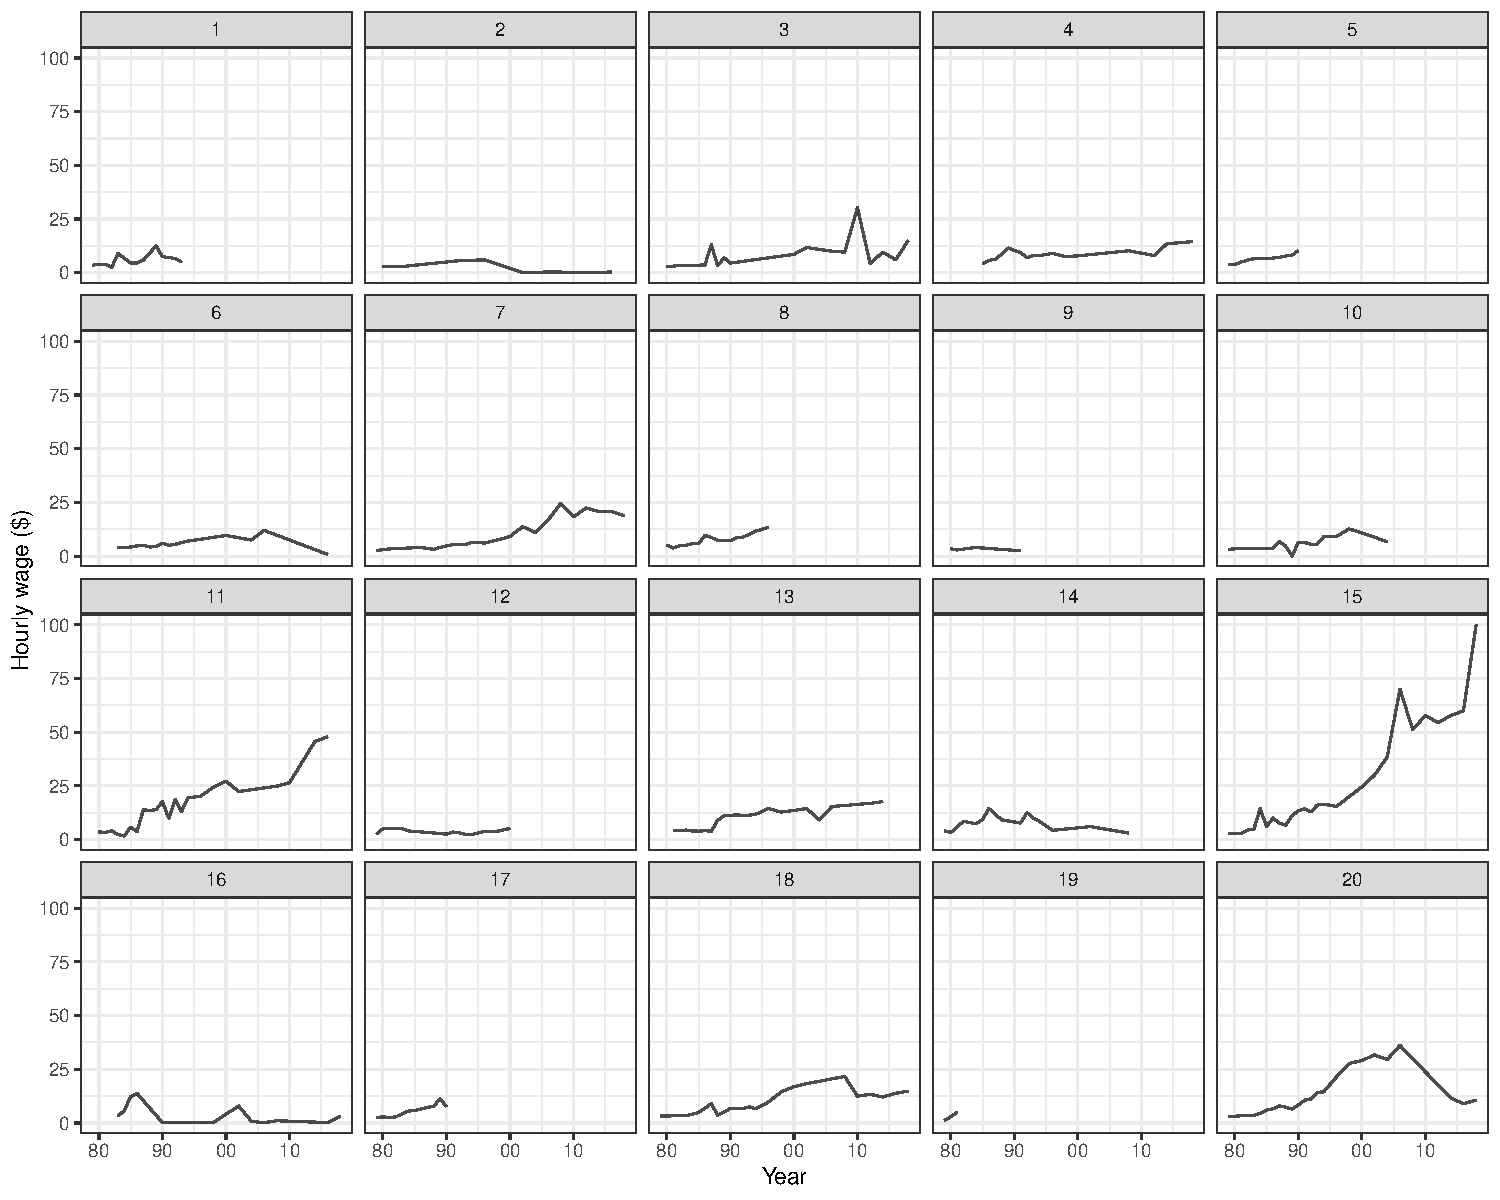
\includegraphics[width=1\linewidth]{figures/sample-plot-1} 

}

\caption{Longitudinal profiles of wages for a random sample of 20 individuals in the refreshed data. Most, but not all, individuals here experienced increasing wages over time, and several have experienced considerable fluctuation in wages. Some individuals are only measured for a short period.}\label{fig:sample-plot}
\end{figure}

We randomly take 20 samples from the data and plot them, as shown in Figure \ref{fig:sample-plot}. It shows that these respondents have a lot of variability in wages, for example, the IDs in panel numbers 5, 7, and 11. The plot also implies that the samples have a different pattern of mean hourly wages. Some have had flat wages for years but had a sudden increase in one particular year, then it gone down again, while the others experienced an upsurge in their wage, for instance, the IDs in panel 9.
However, when checking the summary plots (Figure \ref{fig:feature-plot}), we found that some observations had exceptionally high wages, the maximum value of the wages unbelievably reached about \$60,000/hour. Besides, some of them, for example respondents in Figure \ref {fig:feature-plot} C, had experienced unusual wages only in certain year.

\begin{table}

\caption{\label{tab:age-table}Frequency table of the age at the start of the survey in NSLY79 cohort}
\centering
\begin{tabular}[t]{rr}
\toprule
Age & Number of individuals\\
\midrule
15 & 1,265\\
16 & 1,550\\
17 & 1,600\\
18 & 1,530\\
19 & 1,662\\
20 & 1,722\\
21 & 1,677\\
22 & 1,680\\
\bottomrule
\end{tabular}
\end{table}

\begin{table}

\caption{\label{tab:gender-race-table}Contingency table for gender and race for the full NLSY79 data. The percentage (rounded to closest 1\%) is out of the total corresponding to row.}
\centering
\begin{tabular}[t]{lrrrr}
\toprule
\multicolumn{1}{c}{ } & \multicolumn{3}{c}{Race} & \multicolumn{1}{c}{ } \\
\cmidrule(l{3pt}r{3pt}){2-4}
Gender & Hispanic & Black & Non-Black, Non-Hispanic & Total\\
\midrule
Male & 1,000 (16\%) & 1,613 (25\%) & 3,790 (59\%) & 6,403\\
Female & 1,002 (16\%) & 1,561 (25\%) & 3,720 (59\%) & 6,283\\
\midrule
Total & 2,002 (16\%) & 3,174 (25\%) & 7,510 (59\%) & 12,686\\
\bottomrule
\end{tabular}
\end{table}

\begin{figure}

{\centering 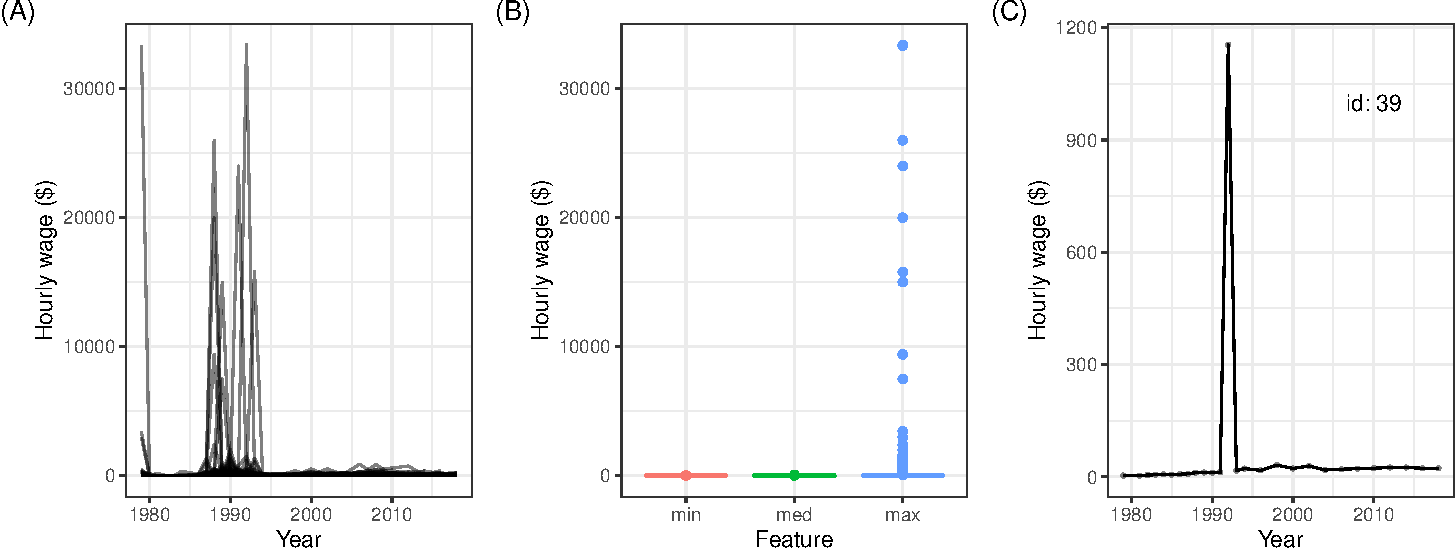
\includegraphics[width=1\linewidth]{figures/feature-plot-1} 

}

\caption{Summary plots to check the data after the tidying stage: (A) longitudinal profiles of wages for all individuals 1979-2018, (B) boxplots of minimum, median, and maximum wages of each individual, (C) and one individual (id=39) with an unusual wage relative to their years of data. It reveals that some values of hourly wages are unbelievable, and some individuals have extemely unusual wages in some years. Accordingly, more cleaning is necessary to treat these extreme values.}\label{fig:feature-plot}
\end{figure}

Extremely high values were also found in the total hours of work, where some observations reported as having worked for 420 hours a week in total. According to Pergamit et al. (2001), one of the flaws of the NLSY79 employment data is that the NLSY79 collects the information of the working hours since the last interview. Thus, it might be challenging for the respondents to track the within-job hours' changes between survey years, especially for the respondents with fluctuating working hours or seasonal jobs. It even has been more challenging since 1994, after which respondents were only surveyed every other year and thus had to recall two full years' job history. This shortcoming might also contribute to the fluctuation of one's wages data.

\hypertarget{censor}{%
\subsection{Replacing extreme values}\label{censor}}

To treat the extreme values in the data, we build a robust linear regression model where we use the robustness weight to determine if a value should be replaced with the fitted value from the model. We build the model for each ID utilizing the \texttt{nest} and \texttt{map} function from \texttt{tidyr} (Wickham 2020) and \texttt{purrr} (Henry and Wickham 2020), respectively. This fits a model separately for each individual, and a robust linear mixed model could be used as an alternative approach. We tried fitting a robust linear mixed model using \texttt{robustlmm} (Koller 2016), however perhaps because the data is large and imbalanced, the model was not converging. The full code for this is shown at \url{CENSORED/articles/input-to-valid-data.html} but also described in detail next.

We build the model using the \texttt{rlm} function from \texttt{MASS} package (Venables and Ripley 2002). We set the \texttt{mean\_hourly\_wage} and \texttt{year} as the dependent and predictor, respectively. Furthermore, we use M-Estimation with Huber weighting, where the observation with a slight residual gets a weight of 1, while the larger the residual, the smaller the weight (less than 1) (UCLA: Statistical Consulting Group 2021). The challenging part of detecting the anomaly using the robustness weight is determining the weight threshold in which the observations are considered outliers. Moreover, it should be noted that not all the outliers are due to an error. Instead, it might be that one had reasonably increasing or decreasing wages in a particular period.

To minimize the risk of mistakenly identifying an outlier as an ``erroneous outlier'', we simulate some thresholds and study how they affect the data by eye balling the results. Based on this eye balling, we find that 0.12 is the most reasonable value to use as the threshold to minimize the risk of overly smoothing the wage by retaining sensible spikes in the data. In other words, we keep maintaining the natural variability of the wages while minimizing anomalies because of the error in the data recording. After deciding the threshold, we impute the observations whose weights are less than 0.12 with the models' predicted value. We then flag those observations in a new variable called \texttt{is\_pred}.

Figure \ref{fig:compare-plot} shows the mean hourly wage before and after the extreme values are replaced. The figure shows that fluctuations in wages still exist even in the imputed data. However, the large spikes, which are considered ``erroneous outliers'', are already eliminated from the data. Hence, the model produces a data set with a more reasonable degree of fluctuation.

\begin{figure}

{\centering 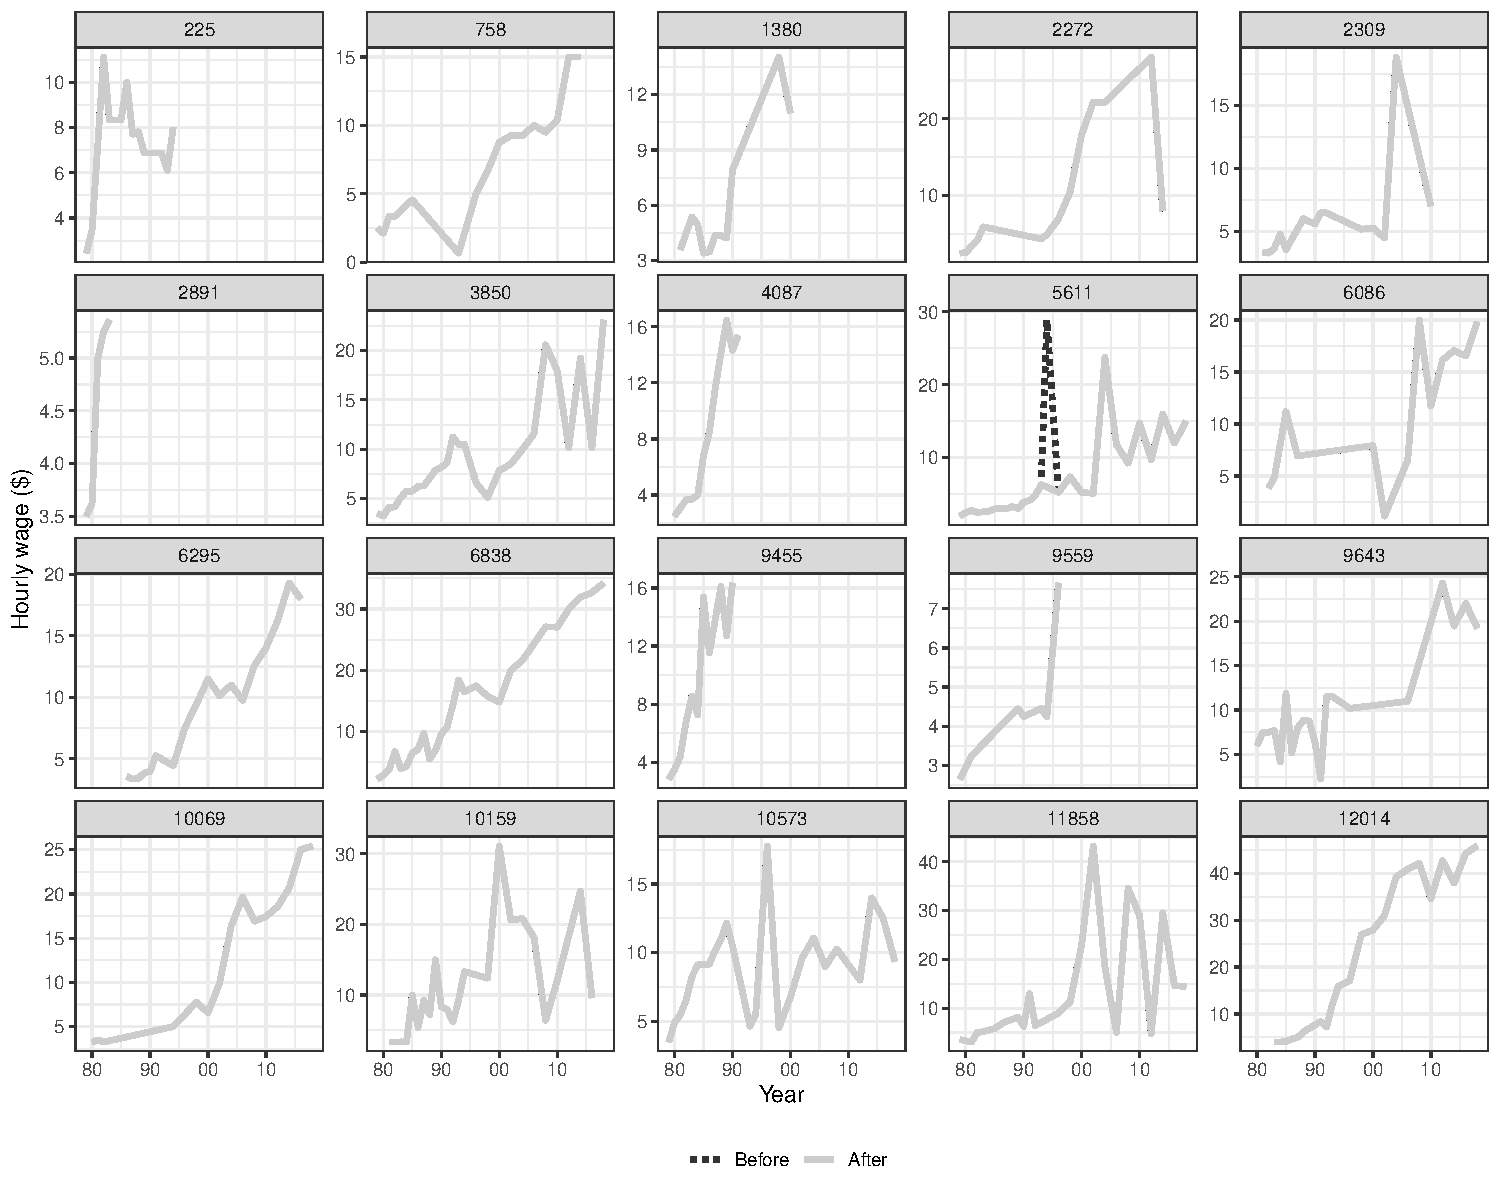
\includegraphics[width=0.9\linewidth]{figures/compare-plot-1} 

}

\caption{Comparison between the original (black dots) and the corrected (solid grey) mean hourly wage for a sample of individuals. A robust linear model prediction was used to correct mean hourly wages value. We can see that some extreme spikes, corresponding to implausible wages, have been replaced with values more similar to wages in neighboring years, but otherwise the profiles are not changed. Some spikes might remain when wage vaues are plausible.}\label{fig:compare-plot}
\end{figure}

Further, Figure \ref{fig:fixed-feature-plot} A shows that after eliminating the extreme values, the highest value has decreased to be around \$350. The spikes are still observed but not as extreme as the original data set. In Figure \ref{fig:fixed-feature-plot} B, we plot the three features of mean hourly wages, namely the minimum, median, and maximum value.
We still can see some extreme values in maximum wages, but consider it as a natural variability of the data. In Figure \ref{fig:fixed-feature-plot} C, we can see that after imputing the extreme value in ID=39, we can see how the the wages change over the years more clearly.

\begin{figure}

{\centering 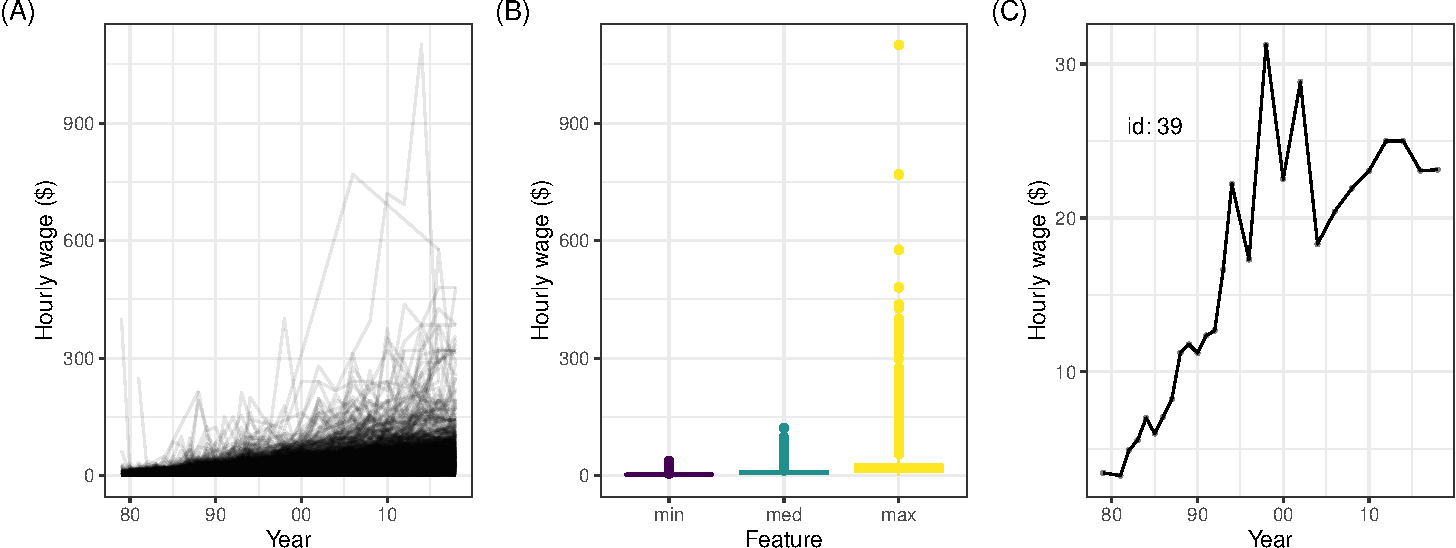
\includegraphics[width=1\linewidth]{figures/fixed-feature-plot-1} 

}

\caption{Re-make of the summary plots of the fully processed data suggest that it is now in a reasonable state: (A) longitudinal profiles of wages for all individuals 1979-2018, (B) boxplots of minimum, median, (C) and maximum wages of each individual, and one individual with an unusual wage relative to their years of data. }\label{fig:fixed-feature-plot}
\end{figure}

Finally, we save the imputed data and set the appropriate data type for the variables.

\hypertarget{recap}{%
\subsection{Recap}\label{recap}}

Figure \ref{fig:flow-chart-blind} summarizes the steps taken to go from raw to input to valid data (M. van der Loo and de Jonge 2018) to create a refreshed wages data set.



\begin{figure}

{\centering 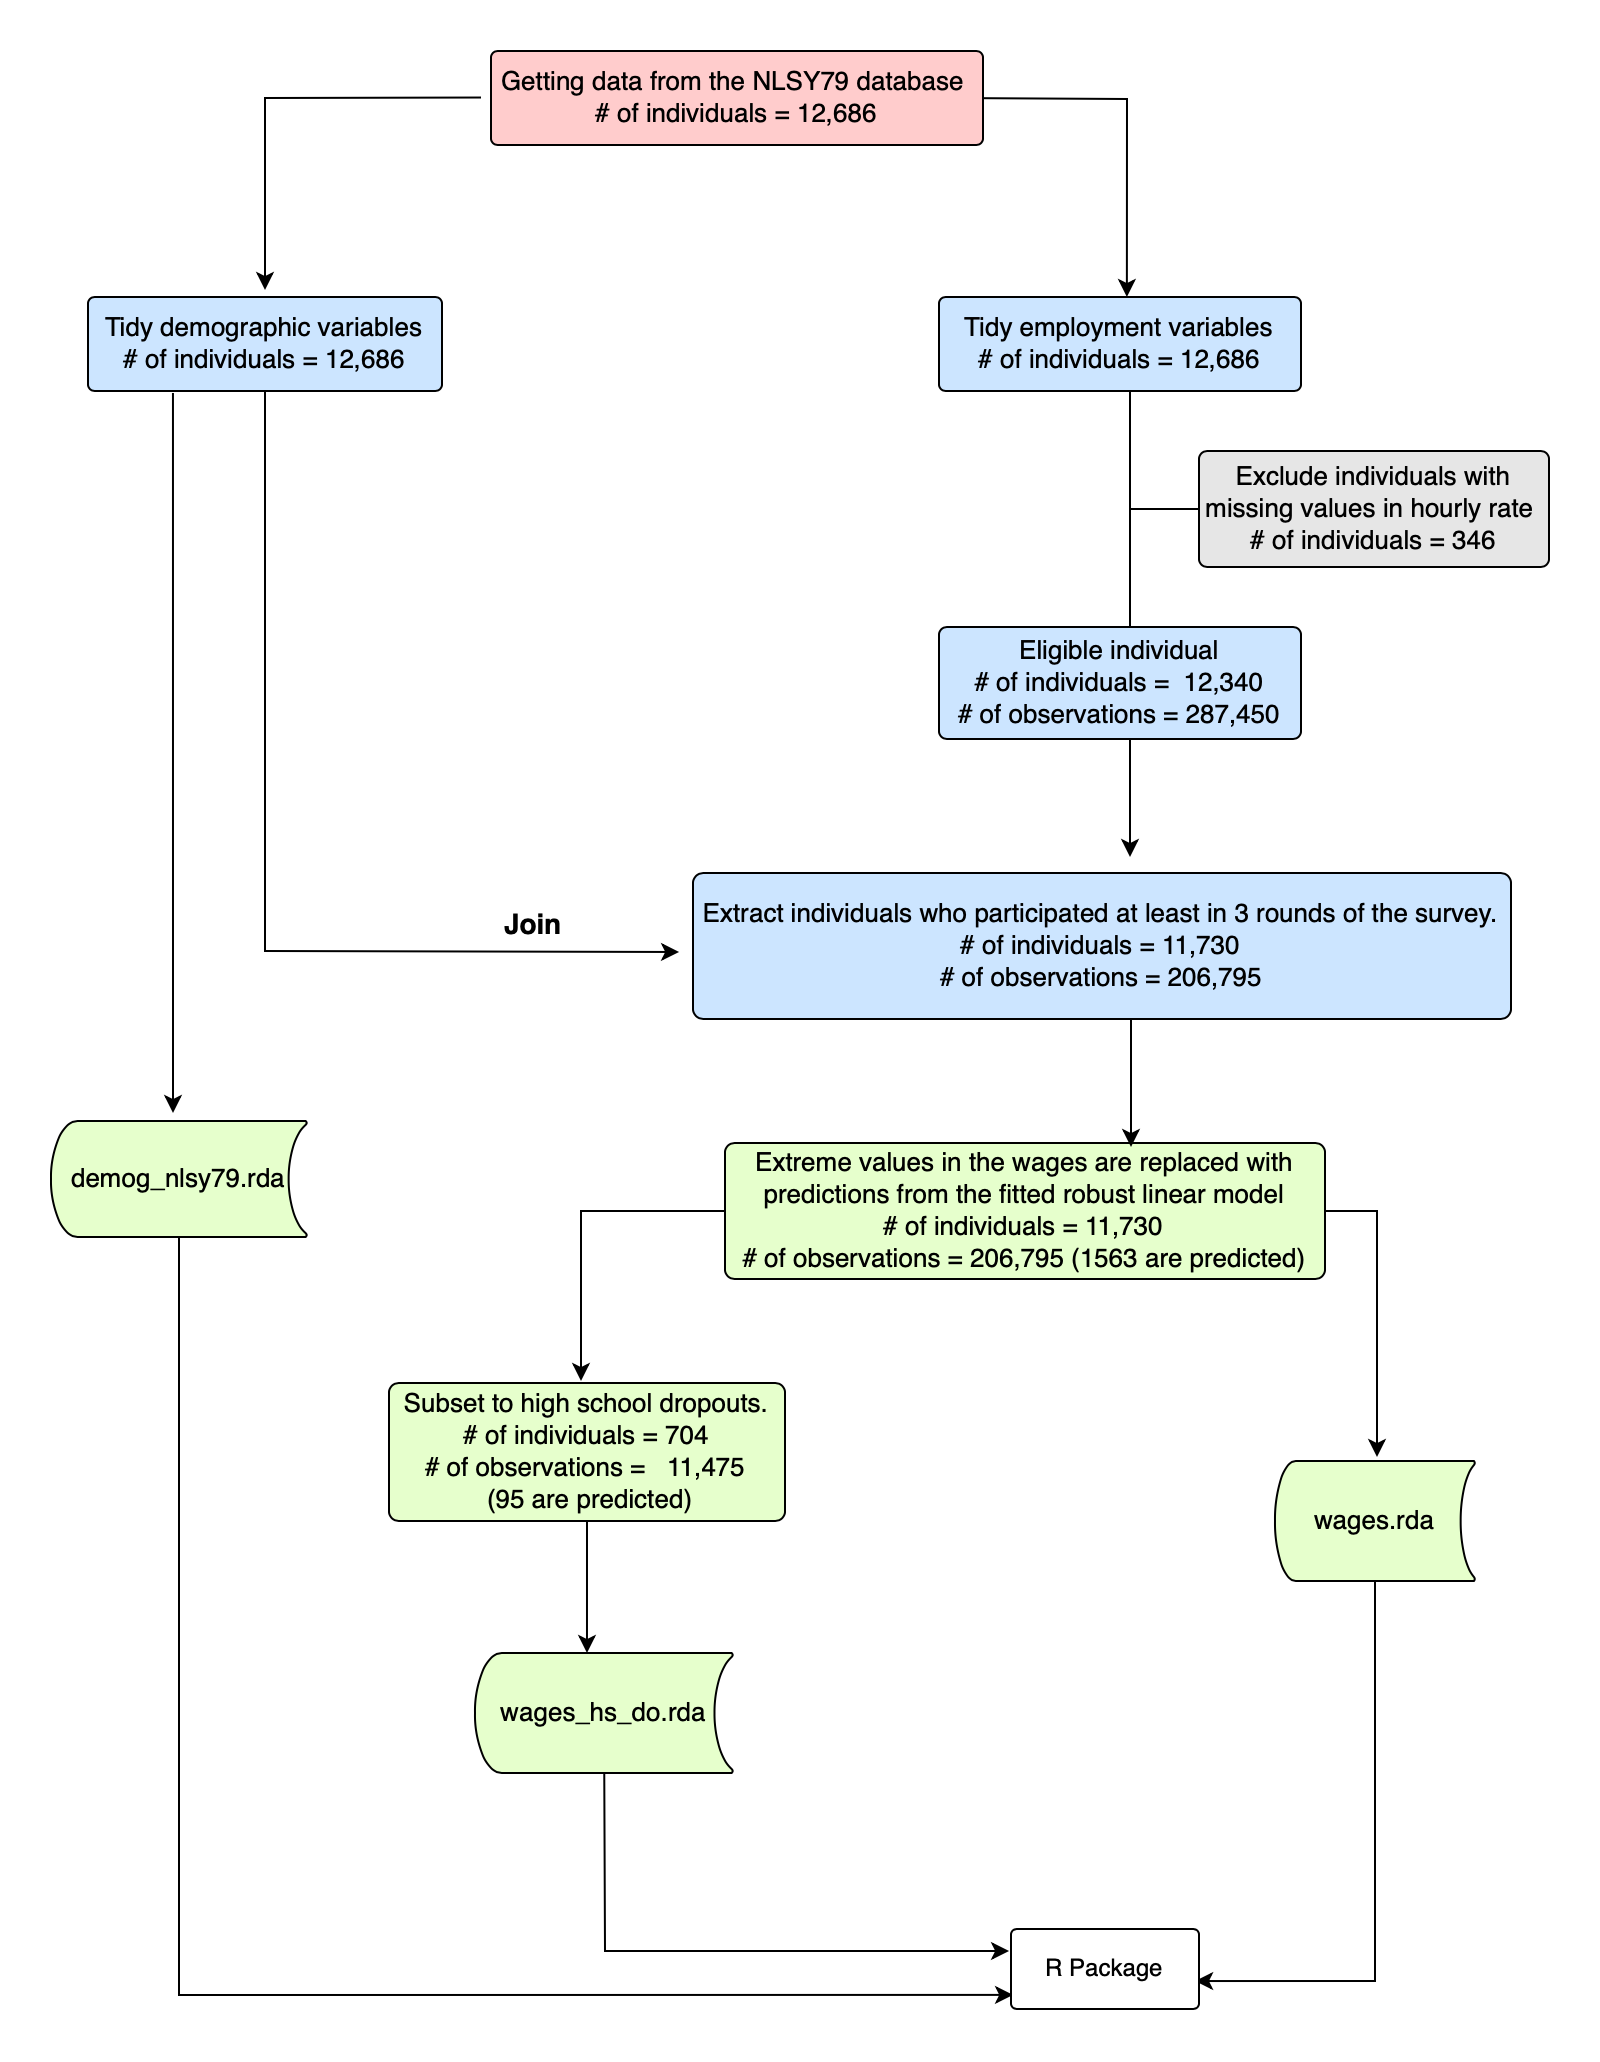
\includegraphics[width=0.85\linewidth]{/Users/cookd/numbats/yowie-paper/paper/figures/flowchart_blind} 

}

\caption{The stages of data cleaning from the raw data to get three datasets contained in \texttt{[CENSORED]}. ``\# of individuals'' means the number of respondents included in each stage, while ``\# of observations'' means the number of rows in the data. The color represents the stage of data cleaning in statistical value chain (M. P. J. van der Loo and de Jonge 2021). Pink, blue, and green represent the raw, input, and valid data, respectively.}\label{fig:flow-chart-blind}
\end{figure}

\hypertarget{compare}{%
\section{Comparison of refreshed with the original data}\label{compare}}

\begin{figure}

{\centering 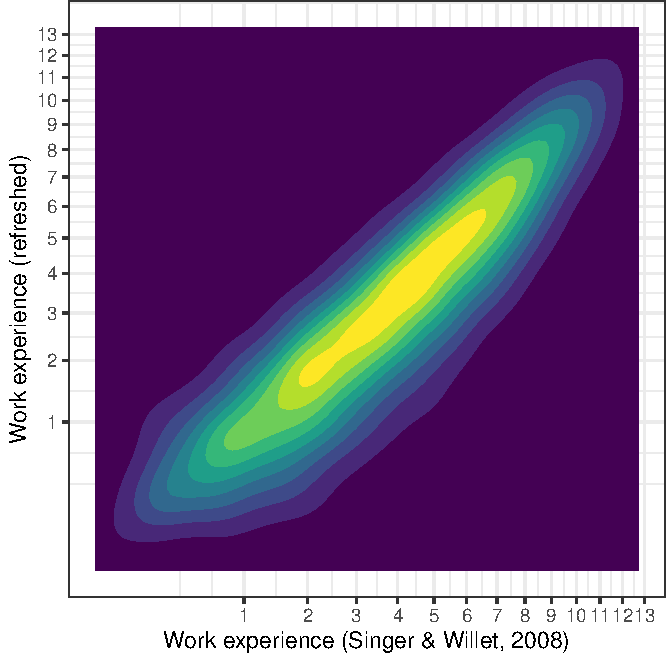
\includegraphics[width=0.7\linewidth]{figures/compare-xp-sw-1} 

}

\caption{Males dropouts' work experience in the original and refreshed data. Each point represents the work experience of individuals (identified by the ID) in the corresponding survey period. We can see that the correlation is reasonably high between them even there are different values for many individuals.}\label{fig:compare-xp-sw}
\end{figure}

The original set contains wages of high school dropouts (Singer and Willett 2003) from 1979 through to 1994. The refreshed data set for comparison is also wages on high school dropouts from 1979 to 2018. The original set is available in the R package \texttt{brolgar} and the refreshed data is available in the R package \texttt{[CENSORED]}.

\hypertarget{filtering-determining-who-is-a-dropout}{%
\subsection{Filtering: Determining who is a dropout}\label{filtering-determining-who-is-a-dropout}}

There is no explicit explanation of how the dropouts cohort is determined in the original data. Hence, we use the high school dropouts criteria from Wolpin (2005), which are:

\begin{enumerate}
\def\labelenumi{\arabic{enumi}.}
\tightlist
\item
  An individual whose highest grade completed (\texttt{hgc}) is reported to be less than 12th grade, \textbf{or}
\item
  An individual whose highest grade completed (\texttt{hgc}) is reported to be at least 12th grade and have received a GED (\texttt{ged} is code to 2).
\end{enumerate}

An additional criteria from Singer and Willett (2003) is to only include males aged between 14 and 17 years old in 1979. With this filtering, we obtained 670 individuals in the refreshed data compared to 888 individuals in the original data. To investigate the reason for the difference, individuals from the original and refreshed dataset were matched by id. This revealed several reasons for for the disparity:

\begin{enumerate}
\def\labelenumi{\arabic{enumi}.}
\tightlist
\item
  173 individuals were more than 17 years old in 1979. Thus, it looks like the description of the original data is not quite accurate, that there are people older than 17 in the subset. Our decision is to also include them in the refreshed data as the new data contains an age variable, so analyst could filter them later.
\item
  79 individuals were less than or equal to 17 years old in 1979. However, they were not captured in the refreshed data because:

  \begin{enumerate}
  \def\labelenumii{\roman{enumii}.}
  \tightlist
  \item
    35 of them completed at least 12th grade with a diploma instead of GED (\texttt{ged} variable is coded to 1). This suggests that they are not dropouts, and so we excluded them from the refreshed data.
  \item
    The information about \texttt{ged} is missing in 38 individuals. We decided to include them in the refreshed data.
  \item
    3 individuals have both diploma and GED (\texttt{ged} is coded to 3). These were kept in the refreshed data.
  \item
    12 individuals do not exist in \texttt{wages} data because they were participated in less than 3 rounds of survey.
  \end{enumerate}
\end{enumerate}

The filtering was re-applied using these decisions, resulting in a refreshed dropout subset containing 863 individuals.

\begin{figure}

{\centering 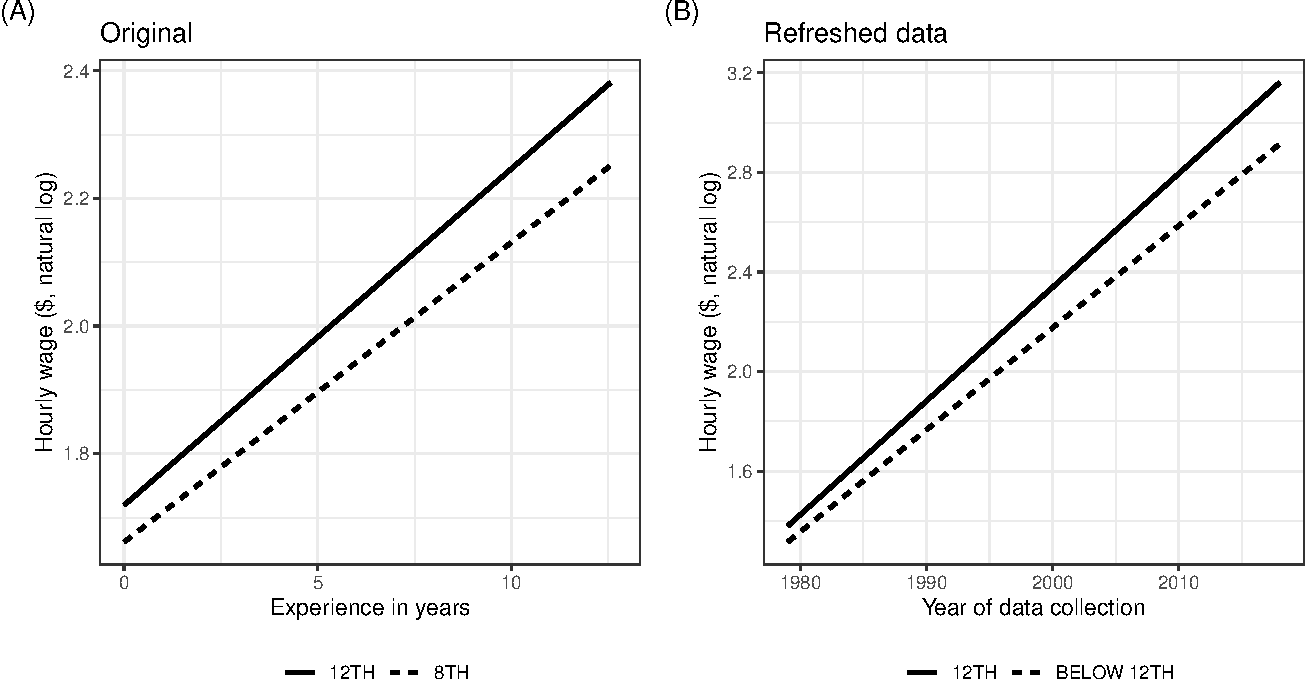
\includegraphics[width=1\linewidth]{figures/plotting-sw-do-1} 

}

\caption{Comparison of original textbook example (A) with refreshed data (B). The original data was inflation-adjusted to 1990 prices and the individual's time of collection was converted to a length of experience in the workforce, which makes it difficult to precisely compare the two sets.}\label{fig:plotting-sw-do}
\end{figure}

\hypertarget{takeaways}{%
\subsection{The takeaways}\label{takeaways}}

There are two aspects of the original data that make the replication with exactly the same result is not obtained. The first one is that the calculation of the time variable provided, which is the ``work experience'', is not clearly articulated. Singer and Willett (2003) mention that the temporal variable is the years of experience since the first day of work. However, this exact same variable is not explicitly available in the database. From the NLSY79 topical guide (Bureau of Labor Statistics, U.S. Department of Labor 2021b), we find that several variables are tagged as work experience-related variables. One of them is the weeks of worked since the last interview. Hence, we use this to calculate the variable. Even though we got different result, the correlation between the original and refreshed work experience is reasonably high as shown in Figure \ref{fig:compare-xp-sw}.

Secondly, in the original dataset, wages were inflation-adjusted to 1990 prices. This is not done for the refreshed data because we plan to keep refreshing it as the data from the newest survey period release. Thus, the 1990 prices might not be relevant anymore for the future context. Hence, we keep it as the original value to allow the users to treat it as their needs.

It is also worth noting that the treatment of unlikely wages differ in the refreshed data. In the original data by Singer and Willett (2003), wages greater than \$75 are set to be missing. However, in recent context, this value is too low to be set as the maximum threshold. We opted to use the weights from a robust linear regression to determine what should be regarded as outliers and imputed them with their predicted values as as described in Section \ref{censor}.

Figure \ref{fig:plotting-sw-do} shows a comparison of the two sets. (A direct ID matching is not possible.) There are 888 individuals in the original and 1,188 individuals in the refreshed data. This suggests some individuals were removed in the original data.
In addition, in the original set the racial breakdown was 246 Black, 204 Hispanic and 438 White participants, while in the refreshed data there are 346 Black, 219 Hispanic, and 623 White participants, so the proportions have not been exactly reproduced. On education, in the refreshed data there are very few individuals with less than a 12th grade education, which is different from the original. In the original data there were 366 individuals with up to 8th grade and 522 9th-12th grade, as compared to 967 with 12th grade in the refreshed data.

\hypertarget{summary}{%
\section{Summary}\label{summary}}

This paper has illustrated the steps and decisions made to take a particular open data set and make it a textbook data set, ready for the classroom or research. In the first stage, we showed the steps performed to get the data from the NLSY79 database. The data format was converted to tidy format, for more flexibility in cleaning and exploring. An initial data analysis was conducted to investigate and screen the quality of the data. We found and provided a fix for many anomalous observations in wages using a robust linear regression model. The refreshed data is compared with the original set using a variety of numerical summaries and graphics. The current subset is made available in a new R package, called \texttt{[CENSORED]}.

The data cleaning process is documented and the code has been made available. These provide the opportunity to again refresh the textbook data as new data is published into the NLSY79 database.
Determining an appropriate robustness weight from which to threshold unusual observations was conducted using a \texttt{shiny} (Chang et al. 2020) app, and the choices used in the refreshed data are documented.

Various difficulties were encountered in trying to refresh the data, which include:

\begin{itemize}
\tightlist
\item
  determining which records should be downloaded from the database.
\item
  calculating experience in the workforce requires comparing the date of first job with the first year the individual was recorded, both of which are available in the database.
\item
  treating the extreme values since there are many unusually high hourly wages, e.g.~greater than \$60,000 per hour.
\item
  determining the dropouts subset as there is no explicit variable in the database recording high school dropout, which means we needed to compare the date of 12th grade with their GED status.
\item
  matching ID's from the original data with those in the refreshed data, do refer to the same person based on the demographic information available.
\end{itemize}

Ultimately, the refreshed data is reasonably similar to the original, but unsatisfactorily far from it. The last step required would be to inflation-adjust wages. This is better to do with each wave of new data added, so that it is relative to the last date in the data. Our decision was to provide the raw wages, and include code to do the adjustment as part of the package.

Some readers may disagree with our decisions made to produce the refreshed textbook data and may have better insight than us in producing a more appropriate textbook data. We do not assert that we have produced the best textbook data, but rather we describe our journey to provide a reasonable textbook data set. All code and documentation are provided for transparency. Readers could use this to make different decisions, or provide suggestions on through package for better choices. Future updates of the \texttt{[CENSORED]} package may contain additional variables, or filters of the full set, if it is deemed important.

For the data providers, we recommend that a better validation system with clear rules applied at data entry, and that alternative output formats, such as a tidy format would help users make better use of their resource. The problem with many of the wages records is that there are implausible values, or confusion on how to record wages for multiple jobs. These values can be validated with simple checks at data entry. Providing an open data resource also is accompanied with the responsibility that the data, especially data that is as valuable as this, is reliable. Users need to be able to trust the data.

Why is this exercise important for teachers and students? This work illustrates the steps in cleaning and processing data in the preparation for it to be a textbook data set. Choices made during the cleaning and processing can affect findings made with the data, and these should be transparent. Along with the textbook data, which is now provided as an R package, the documentation of the process provide some examples for teaching data cleaning, initial data analysis and exploratory data analysis. The refreshed textbook data provides a resource for teaching longitudinal data analysis.

The wages data provides a good opportunity to discuss the difference between statistics to use for public policy and statistics that relate to the individual. Public policy is based on models, yielding averages that might vary across strata. Modeling the wages relative to workforce experience, with demographic covariates we learn that there are significantly different patterns. That more education leads to increasingly higher wages, which is a satisfying result for educators. It means that education makes a difference in the wage experience, and that public policy that encourages education is a data-supported action. We would also learn, although not presented here, that race matters and that being black leads to lower wages. This is a disturbing finding because there is no rational for such a difference in a fair society. This would provide support for action in public policy to remove this overall average effect. It also provides an example for educators to explain the use of data to support public policy action.

On an individual level, one needs to know where am I in this data, and does this data relate to me. To do this, the individual profiles need to be explored. Pre-dominantly, we would learn that the variation from one individual to another is far more than the variation between demographic strata. For example, many individuals with lower educational attainment earn very high wages. From a statistics and data science educator perspective, more focus and more methodology for this type of statistics needs to be included in the curriculum.

The above interpretations of results from analyzing the wages data, rely on trusting that the data provided is accurate and valid. The wages data is collected by a reputable organization, but we found that the data has obvious errors that should be corrected. This paper has illustrated procedures and guidelines to achieve valid data, and provides the code and details for it to be reproduced, and modified if deemed appropriate.

Having trustworthy data is imperative for statistics and data science education. Whenever one uses a textbook data set that is perceived as relating to the students lives, there will be interpretations made. The wages data is an example of this. Students will take away the interpretations from whatever is taught with the data, that wages increase with experience, education, race. If one uses data examples that are synthetic, instilled with our own inherent prejudices (for e.g.~gender and race), or data that has been poorly processed containing errors, we as educators are being irresponsible because the societal message taught to students may be flawed. This paper demonstrates the process to produce a trustworthy data set for teaching.

\hypertarget{acknowledgements}{%
\section{Acknowledgements}\label{acknowledgements}}

We would like to thank Aarathy Babu for the insight and discussion during the writing of this paper.

The entire analysis is conducted using \texttt{R} (R Core Team 2020) in RStudio IDE using these packages: \texttt{tidyverse} (Wickham et al. 2019), \texttt{ggplot2} (Wickham 2016), \texttt{dplyr} (Wickham et al. 2020), \texttt{readr} (Wickham and Hester 2020), \texttt{tidyr} (Wickham 2020), \texttt{stringr} (Wickham 2019), \texttt{purrr} (Henry and Wickham 2020), \texttt{brolgar} (Tierney, Cook, and Prvan 2020), \texttt{patchwork} (Pedersen 2020), \texttt{kableExtra} (Zhu 2019), \texttt{MASS} (Venables and Ripley 2002), \texttt{janitor} (Firke 2020), and \texttt{tsibble} (Wang, Cook, and Hyndman 2020). The paper was generated using \texttt{knitr} (Xie 2014) and \texttt{rmarkdown} (Xie, Dervieux, and Riederer 2020).

\hypertarget{supplementary-materials}{%
\section{Supplementary Materials}\label{supplementary-materials}}

\begin{itemize}
\item
  \textbf{Codes}: R script to reproduce data tidying and cleaning is available in this \href{CENSORED/articles/process-data.html}{page}.
\item
  \textbf{R Package}:\texttt{[CENSORED]} is a data container R package that contains 3 datasets, namely the high school mean hourly wage data, high school dropouts mean hourly wage data, and demographic data of the NLSY79 cohort. This package can be accessed \href{CENSORED}{here}.
\item
  \textbf{shiny app}: An interactive \texttt{shiny} web app to visualise the effect of selecting different weight threshold for substituting the wages data to its predicted value from a fit of the robust linear regression model. This app can be accessed \href{CENSORED}{here} with the source code provided \href{CENSORED/tree/master/app}{here}.
\end{itemize}

\hypertarget{data-availability-statement}{%
\section{Data Availability Statement}\label{data-availability-statement}}

The authors confirm that the data supporting the findings of this study are available within the supplementary materials.

\hypertarget{references}{%
\section*{References}\label{references}}
\addcontentsline{toc}{section}{References}

\hypertarget{refs}{}
\begin{CSLReferences}{1}{0}
\leavevmode\vadjust pre{\hypertarget{ref-iris-data}{}}%
Andereson, Edgar. 1935. {``The Irises of the Gaspe Peninsula.''} \emph{Bulletin of the American Iris Society} 59: 2--5.

\leavevmode\vadjust pre{\hypertarget{ref-nlsy79}{}}%
Bureau of Labor Statistics, U.S. Department of Labor. 2021a. {``National Longitudinal Survey of Youth 1979 Cohort, 1979-2016 (Rounds 1-28).''} Produced and distributed by the Center for Human Resource Research (CHRR), The Ohio State University. Columbus, OH, through \url{https://www.nlsinfo.org/bibliography-citing-nls-data}.

\leavevmode\vadjust pre{\hypertarget{ref-nlsy79guide}{}}%
---------. 2021b. {``National Longitudinal Survey of Youth 1979 Cohort, Topical Guide to the Data.''} \url{https://www.nlsinfo.org/content/cohorts/nlsy79/topical-guide/employment/work-experience}.

\leavevmode\vadjust pre{\hypertarget{ref-shiny}{}}%
Chang, Winston, Joe Cheng, JJ Allaire, Yihui Xie, and Jonathan McPherson. 2020. \emph{{shiny: Web Application Framework for R}}. \url{https://CRAN.R-project.org/package=shiny}.

\leavevmode\vadjust pre{\hypertarget{ref-Chatfield1985TIEo}{}}%
Chatfield, C. 1985. {``The Initial Examination of Data.''} \emph{Journal of the Royal Statistical Society. Series A. General} 148 (3): 214--53.

\leavevmode\vadjust pre{\hypertarget{ref-eliznlsy}{}}%
Cooksey, Elizabeth C. 2017. {``Using the National Longitudinal Surveys of Youth (NLSY) to Conduct Life Course Analyses.''} In \emph{Handbook of Life Course Health Development}, edited by Richard M. Lerner Neal Halfon Christoper B. Forrest, 561--77. Cham: Springer. https://doi.org/\url{https://doi.org/10.1007/978-3-319-47143-3_23}.

\leavevmode\vadjust pre{\hypertarget{ref-DasuTamraparni2003Edma}{}}%
Dasu, Tamraparni, and Theodore Johnson. 2003. \emph{Exploratory Data Mining and Data Cleaning}. Wiley Series in Probability and Statistics. Hoboken: WILEY.

\leavevmode\vadjust pre{\hypertarget{ref-janitor}{}}%
Firke, Sam. 2020. \emph{{janitor: Simple Tools for Examining and Cleaning Dirty Data}}. \url{https://CRAN.R-project.org/package=janitor}.

\leavevmode\vadjust pre{\hypertarget{ref-racismnotrace}{}}%
Fullilove, M. T. 1998. {``Comment: Abandoning ``Race" as a Variable in Public Health Research--an Idea Whose Time Has Come.''} \emph{American Journal of Public Health} 88 (9): 1297--98.

\leavevmode\vadjust pre{\hypertarget{ref-grimshaw}{}}%
Grimshaw, Scott D. 2015. {``A Framework for Infusing Authentic Data Experiences Within Statistics Courses.''} \emph{The American Statistician} 69 (4): 307--14. \url{https://doi.org/10.1080/00031305.2015.1081106}.

\leavevmode\vadjust pre{\hypertarget{ref-purrr}{}}%
Henry, Lionel, and Hadley Wickham. 2020. \emph{{purrr: Functional Programming Tools}}. \url{https://CRAN.R-project.org/package=purrr}.

\leavevmode\vadjust pre{\hypertarget{ref-penguins-data}{}}%
Horst, Allison Marie, Alison Presmanes Hill, and Kristen B Gorman. 2020. \emph{Palmerpenguins: Palmer Archipelago (Antarctica) Penguin Data}. \url{https://doi.org/10.5281/zenodo.3960218}.

\leavevmode\vadjust pre{\hypertarget{ref-HuebnerMariannePhD2016Asat}{}}%
Huebner, Marianne, Werner Vach, and Saskia le Cessie. 2016. {``A Systematic Approach to Initial Data Analysis Is Good Research Practice.''} \emph{The Journal of Thoracic and Cardiovascular Surgery} 151 (1): 25--27.

\leavevmode\vadjust pre{\hypertarget{ref-ilk2004}{}}%
Ilk, Ozlem. 2004. {``Exploratory Multivariate Longitudinal Data Analysis and Models for Multivariate Longitudinal Binary Data.''} PhD thesis, Iowa State University. \url{https://doi.org/10.31274/rtd-180813-11012}.

\leavevmode\vadjust pre{\hypertarget{ref-tamedata}{}}%
Kim, A. Y, C. Ismay, and J. Chunn. 2018. {``The Fivethirtyeight {R} Package: ``Tame Data" Principles for Introductory Statistics and Data Science Courses.''} \emph{Technology Innovations in Statistics Education} 11 (1). \url{https://doi.org/10.5070/T511103589}.

\leavevmode\vadjust pre{\hypertarget{ref-KollerManuel2016rARP}{}}%
Koller, Manuel. 2016. {``{robustlmm: An R Package for Robust Estimation of Linear Mixed-Effects Models}.''} \emph{Journal of Statistical Software} 75 (6): 1--24.

\leavevmode\vadjust pre{\hypertarget{ref-notaverage}{}}%
Moncrief, Marc. 2015. {``By the Numbers - the Average Australian Doesn't Exist ... Not a Single One of Us Is 'Normal'.''} \url{https://bit.ly/smh-not-normal}.

\leavevmode\vadjust pre{\hypertarget{ref-opendata}{}}%
Open Knowledge Foundation. 2021. {``Open Definition. Defining Open in Open Data, Open Content, and Open Knowledge.''} 2021. \url{http://opendefinition.org/od/2.1/en/}.

\leavevmode\vadjust pre{\hypertarget{ref-patchwork}{}}%
Pedersen, Thomas Lin. 2020. \emph{{patchwork: The Composer of Plots}}. \url{https://CRAN.R-project.org/package=patchwork}.

\leavevmode\vadjust pre{\hypertarget{ref-MichaelRPergamit2001DWTN}{}}%
Pergamit, Michael R., Charles R. Pierret, Donna S. Rothstein, and Jonathan R. Veum. 2001. {``Data Watch: The National Longitudinal Surveys.''} \emph{The Journal of Economic Perspectives} 15 (2): 239--53.

\leavevmode\vadjust pre{\hypertarget{ref-R}{}}%
R Core Team. 2020. \emph{R: A Language and Environment for Statistical Computing}. Vienna, Austria: R Foundation for Statistical Computing. \url{https://www.R-project.org/}.

\leavevmode\vadjust pre{\hypertarget{ref-SingerJudithD2003Alda}{}}%
Singer, Judith D, and John B Willett. 2003. \emph{Applied Longitudinal Data Analysis: Modeling Change and Event Occurrence}. Oxford u.a: Oxford Univ. Pr.

\leavevmode\vadjust pre{\hypertarget{ref-notiris}{}}%
Stodel, Megan. 2020. {``Stop Using Iris.''} \url{https://www.meganstodel.com/posts/no-to-iris/}.

\leavevmode\vadjust pre{\hypertarget{ref-brolgar}{}}%
Tierney, Nicholas, Di Cook, and Tania Prvan. 2020. \emph{{brolgar: BRowse Over Longitudinal data Graphically and Analytically in R}}. \url{https://github.com/njtierney/brolgar}.

\leavevmode\vadjust pre{\hypertarget{ref-tukey}{}}%
Tukey, John W. (John Wilder). 1977. \emph{Exploratory Data Analysis}. Addison-Wesley Series in Behavioral Science. Reading, Mass.: Addison-Wesley Pub. Co.

\leavevmode\vadjust pre{\hypertarget{ref-rlm}{}}%
UCLA: Statistical Consulting Group. 2021. {``{Robust Regression \textbar{} R Data Analysis Examples}.''} February 2021. \url{https://stats.idre.ucla.edu/r/dae/robust-regression/}.

\leavevmode\vadjust pre{\hypertarget{ref-validate}{}}%
van der Loo, Mark P. J., and Edwin de Jonge. 2021. {``Data Validation Infrastructure for {R}.''} \emph{Journal of Statistical Software} 97 (10): 1--31. \url{https://doi.org/10.18637/jss.v097.i10}.

\leavevmode\vadjust pre{\hypertarget{ref-LooMarkvander2018Sdcw}{}}%
van der Loo, Mark, and Edwin de Jonge. 2018. \emph{Statistical Data Cleaning with Applications in r}.

\leavevmode\vadjust pre{\hypertarget{ref-mass}{}}%
Venables, W. N., and B. D. Ripley. 2002. \emph{Modern Applied Statistics with s}. Fourth. New York: Springer. \url{http://www.stats.ox.ac.uk/pub/MASS4}.

\leavevmode\vadjust pre{\hypertarget{ref-tsibble}{}}%
Wang, Earo, Dianne Cook, and Rob J Hyndman. 2020. {``A New Tidy Data Structure to Support Exploration and Modeling of Temporal Data.''} \emph{Journal of Computational and Graphical Statistics} 29 (3): 466--78. \url{https://doi.org/10.1080/10618600.2019.1695624}.

\leavevmode\vadjust pre{\hypertarget{ref-plyr}{}}%
Wickham, Hadley. 2011. {``The Split-Apply-Combine Strategy for Data Analysis.''} \emph{Journal of Statistical Software, Articles} 40 (1): 1--29. \url{https://doi.org/10.18637/jss.v040.i01}.

\leavevmode\vadjust pre{\hypertarget{ref-WickhamHadley2014TD}{}}%
---------. 2014. {``Tidy Data.''} \emph{Journal of Statistical Software} 59 (10): 1--23.

\leavevmode\vadjust pre{\hypertarget{ref-ggplot2}{}}%
---------. 2016. \emph{{ggplot2: Elegant Graphics for Data Analysis}}. Springer-Verlag New York. \url{https://ggplot2.tidyverse.org}.

\leavevmode\vadjust pre{\hypertarget{ref-stringr}{}}%
---------. 2019. \emph{{stringr: Simple, Consistent Wrappers for Common String Operations}}. \url{https://CRAN.R-project.org/package=stringr}.

\leavevmode\vadjust pre{\hypertarget{ref-tidyr}{}}%
---------. 2020. \emph{{tidyr: Tidy Messy Data}}. \url{https://CRAN.R-project.org/package=tidyr}.

\leavevmode\vadjust pre{\hypertarget{ref-tidyverse}{}}%
Wickham, Hadley, Mara Averick, Jennifer Bryan, Winston Chang, Lucy D'Agostino McGowan, Romain François, Garrett Grolemund, et al. 2019. {``Welcome to the {tidyverse}.''} \emph{Journal of Open Source Software} 4 (43): 1686. \url{https://doi.org/10.21105/joss.01686}.

\leavevmode\vadjust pre{\hypertarget{ref-dplyr}{}}%
Wickham, Hadley, Romain François, Lionel Henry, and Kirill Müller. 2020. \emph{{dplyr: A Grammar of Data Manipulation}}. \url{https://CRAN.R-project.org/package=dplyr}.

\leavevmode\vadjust pre{\hypertarget{ref-readr}{}}%
Wickham, Hadley, and Jim Hester. 2020. \emph{{readr: Read Rectangular Text Data}}. \url{https://CRAN.R-project.org/package=readr}.

\leavevmode\vadjust pre{\hypertarget{ref-nlsy79edu}{}}%
Wolpin, Kenneth I. 2005. {``National Longitudinal Survey of Youth 1979 Cohort, 1979-2016 (Rounds 1-28).''} Published by Bureau of Labor Statistics, U.S. Department of Labor. \url{https://www.bls.gov/opub/mlr/2005/02/art3full.pdf}.

\leavevmode\vadjust pre{\hypertarget{ref-knitr}{}}%
Xie, Yihui. 2014. {``Knitr: A Comprehensive Tool for Reproducible Research in {R}.''} In \emph{Implementing Reproducible Computational Research}, edited by Victoria Stodden, Friedrich Leisch, and Roger D. Peng. Chapman; Hall/CRC. \url{http://www.crcpress.com/product/isbn/9781466561595}.

\leavevmode\vadjust pre{\hypertarget{ref-rmarkdown}{}}%
Xie, Yihui, Christophe Dervieux, and Emily Riederer. 2020. \emph{R Markdown Cookbook}. Boca Raton, Florida: Chapman; Hall/CRC. \url{https://bookdown.org/yihui/rmarkdown-cookbook}.

\leavevmode\vadjust pre{\hypertarget{ref-kableExtra}{}}%
Zhu, Hao. 2019. \emph{{kableExtra: Construct Complex Table with 'kable' and Pipe Syntax}}. \url{https://CRAN.R-project.org/package=kableExtra}.

\end{CSLReferences}

\bibliographystyle{unsrt}
\bibliography{references.bib}


\end{document}
